%package list
\documentclass{article}
\usepackage[top=3cm, bottom=3cm, outer=3cm, inner=3cm]{geometry}
\usepackage{multicol}
\usepackage{graphicx}
\usepackage{url}
%\usepackage{cite}
\usepackage{hyperref}
\usepackage{array}
%\usepackage{multicol}
\newcolumntype{x}[1]{>{\centering\arraybackslash\hspace{0pt}}p{#1}}
\usepackage{natbib}
\usepackage{pdfpages}
\usepackage{multirow}    
\usepackage[normalem]{ulem}
\useunder{\uline}{\ul}{}
\usepackage{svg}
\usepackage{xcolor}
\usepackage{listings}
\lstdefinestyle{ascii-tree}{
    literate={├}{|}1 {─}{--}1 {└}{+}1 
  }

\lstset{basicstyle=\ttfamily,
  showstringspaces=false,
  commentstyle=\color{red},
  keywordstyle=\color{blue}
}
%\usepackage{booktabs}
\usepackage{caption}
\usepackage{subcaption}
\usepackage{float}
\usepackage{array}

\usepackage{enumitem}


\newcolumntype{M}[1]{>{\centering\arraybackslash}m{#1}}
\newcolumntype{N}{@{}m{0pt}@{}}


%%%%%%%%%%%%%%%%%%%%%%%%%%%%%%%%%%%%%%%%%%%%%%%%%%%%%%%%%%%%%%%%%%%%%%%%%%%%
%%%%%%%%%%%%%%%%%%%%%%%%%%%%%%%%%%%%%%%%%%%%%%%%%%%%%%%%%%%%%%%%%%%%%%%%%%%%
\newcommand{\itemEmail}{vmaldonadov@unsa.edu.pe}
\newcommand{\itemStudent}{Victor Gonzalo Maldonado Vilca}
\newcommand{\itemCourse}{Programación Web 2}
\newcommand{\itemCourseCode}{1702122}
\newcommand{\itemSemester}{III}
\newcommand{\itemUniversity}{Universidad Nacional de San Agustín de Arequipa}
\newcommand{\itemFaculty}{Facultad de Ingeniería de Producción y Servicios}
\newcommand{\itemDepartment}{Departamento Académico de Ingeniería de Sistemas e Informática}
\newcommand{\itemSchool}{Escuela Profesional de Ingeniería de Sistemas}
\newcommand{\itemAcademic}{2024 - A}
\newcommand{\itemInput}{Del 23 de mayo de 2024}
\newcommand{\itemOutput}{Al 8 de julio de 2024}
\newcommand{\itemPracticeNumber}{10}
\newcommand{\itemTheme}{Angular 2}
%%%%%%%%%%%%%%%%%%%%%%%%%%%%%%%%%%%%%%%%%%%%%%%%%%%%%%%%%%%%%%%%%%%%%%%%%%%%
%%%%%%%%%%%%%%%%%%%%%%%%%%%%%%%%%%%%%%%%%%%%%%%%%%%%%%%%%%%%%%%%%%%%%%%%%%%%

\usepackage[english,spanish]{babel}
\usepackage[utf8]{inputenc}
\AtBeginDocument{\selectlanguage{spanish}}
\renewcommand{\figurename}{Figura}
\renewcommand{\refname}{Referencias}
\renewcommand{\tablename}{Tabla} %esto no funciona cuando se usa babel
\AtBeginDocument{%
	\renewcommand\tablename{Tabla}
}

\usepackage{fancyhdr}
\pagestyle{fancy}
\fancyhf{}
\setlength{\headheight}{30pt}
\renewcommand{\headrulewidth}{1pt}
\renewcommand{\footrulewidth}{1pt}
\fancyhead[L]{\raisebox{-0.2\height}{
\includegraphics[width=3cm]{img/logo_episunsa.png}}}
\fancyhead[C]{\fontsize{7}{7}\selectfont	\itemUniversity \\ \itemFaculty \\ \itemDepartment \\ \itemSchool \\ \textbf{\itemCourse}}
\fancyhead[R]{\raisebox{-0.2\height}{
\includegraphics[width=1.2cm]{img/logo_abet}}}
\fancyfoot[L]{Victor M.}
\fancyfoot[C]{\itemCourse}
\fancyfoot[R]{Página \thepage}

% para el codigo fuente
\usepackage{listings}
\usepackage{color, colortbl}
\definecolor{dkgreen}{rgb}{0,0.6,0}
\definecolor{gray}{rgb}{0.5,0.5,0.5}
\definecolor{mauve}{rgb}{0.58,0,0.82}
\definecolor{codebackground}{rgb}{0.95, 0.95, 0.92}
\definecolor{tablebackground}{rgb}{0.8, 0, 0}

\lstset{frame=tb,
	language=bash,
	aboveskip=3mm,
	belowskip=3mm,
	showstringspaces=false,
	columns=flexible,
	basicstyle={\small\ttfamily},
	numbers=none,
	numberstyle=\tiny\color{gray},
	keywordstyle=\color{blue},
	commentstyle=\color{dkgreen},
	stringstyle=\color{mauve},
	breaklines=true,
	breakatwhitespace=true,
	tabsize=3,
	backgroundcolor= \color{codebackground},
}

\begin{document}
	
	\vspace*{10px}
	
	\begin{center}	
		\fontsize{17}{17} \textbf{ Informe de Angular 2 }
	\end{center}
	\centerline{\textbf{\Large Tema: \itemTheme}}
	%\vspace*{0.5cm}	

	\begin{flushright}
		\begin{tabular}{|M{2.5cm}|N|}
			\hline 
			\rowcolor{tablebackground}
			\color{white} \textbf{Nota}  \\
			\hline 
			     \\[30pt]
			\hline 			
		\end{tabular}
	\end{flushright}	

	\begin{table}[H]
		\begin{tabular}{|x{4.7cm}|x{4.8cm}|x{4.8cm}|}
			\hline 
			\rowcolor{tablebackground}
			\color{white} \textbf{Estudiante} & \color{white}\textbf{Escuela}  & \color{white}\textbf{Asignatura}   \\
			\hline 
			{\itemStudent \par \itemEmail} & \itemSchool & {\itemCourse \par Semestre: \itemSemester \par Código: \itemCourseCode}     \\
			\hline 			
		\end{tabular}
	\end{table}		
	
	\begin{table}[H]
		\begin{tabular}{|x{4.7cm}|x{4.8cm}|x{4.8cm}|}
			\hline 
			\rowcolor{tablebackground}
			\color{white}\textbf{Tarea} & \color{white}\textbf{Tema}  & \color{white}\textbf{Duración}   \\
			\hline 
			\itemPracticeNumber & \itemTheme & 2 horas   \\
			\hline 
		\end{tabular}
	\end{table}
	
	\begin{table}[H]
		\begin{tabular}{|x{4.7cm}|x{4.8cm}|x{4.8cm}|}
			\hline 
			\rowcolor{tablebackground}
			\color{white}\textbf{Semestre académico} & \color{white}\textbf{Fecha de inicio}  & \color{white}\textbf{Fecha de entrega}   \\
			\hline 
			\itemAcademic & \itemInput &  \itemOutput  \\
			\hline 
		\end{tabular}
	\end{table}
%%%%%%%%%%%%%%%%%%%%

  \section{Introducción}
  Angular es un framework desarrollado por Google para crear aplicaciones web y móviles robustas y escalables. 
  Se destaca por su arquitectura basada en componentes, enlace de datos bidireccional, y herramientas integradas 
  para manejar formularios, enrutamiento y optimización de rendimiento. Es ampliamente utilizado por su capacidad 
  de desarrollar aplicaciones de una sola página (SPAs) de manera eficiente y estructurada.

%%%%%%%%%%%%%%%%%%%%

  \section{Objetivos}
  \begin{itemize}
    \item Manejar el sistema de ruteos que ofrece Angular.
    \item Visualizar que otras aplicaciones tiene Angular.
    \item Entender conceptos de BackEnd y FrontEnd.
    \item Manejar Módulos, Componentes y Servicios.
  \end{itemize}

%%%%%%%%%%%%%%%%%%%%
 
	\section{Tarea}
  \begin{itemize}
    \item Volver a implementar las clases teóricas en un proyecto en github realizando commits de cada avance.  
    \item Compartirlo con el profesor (usuario CarloCorrales010)
  \end{itemize}
  
%%%%%%%%%%%%%%%%%%%% 
 
  \section{Entregables}
  \begin{itemize}
    \item Informe hecho en Latex.
    \item URL: Repositorio GitHub.
  \end{itemize}
  
%%%%%%%%%%%%%%%%%%%%    
		
	\section{Equipos, materiales y temas utilizados}
  \begin{itemize}
    \item Angular
    \item Componentes
    \item Servicios
    \item Formularios y Referencias
    \item Boostrap
    \item Django
  \end{itemize}
 
%%%%%%%%%%%%%%%%%%%%

  \section{URL de Repositorio Github}
  \begin{itemize}
    \item Link Repositorio GitHub.
    \item \url{https://github.com/Victor-Gonzalo-Maldonado-Vilca/Angular.git}
  \end{itemize}

%%%%%%%%%%%%%%%%%%%%

  \section{Desarrollo del trabajo}
  \textit{Continuamos con el Desarrollo a partir de Angular1}
  
%%%%%%%%%%%%

  \subsection{Capturas de la Actividad}
  \begin{figure}[H]
    \centering
    \fbox{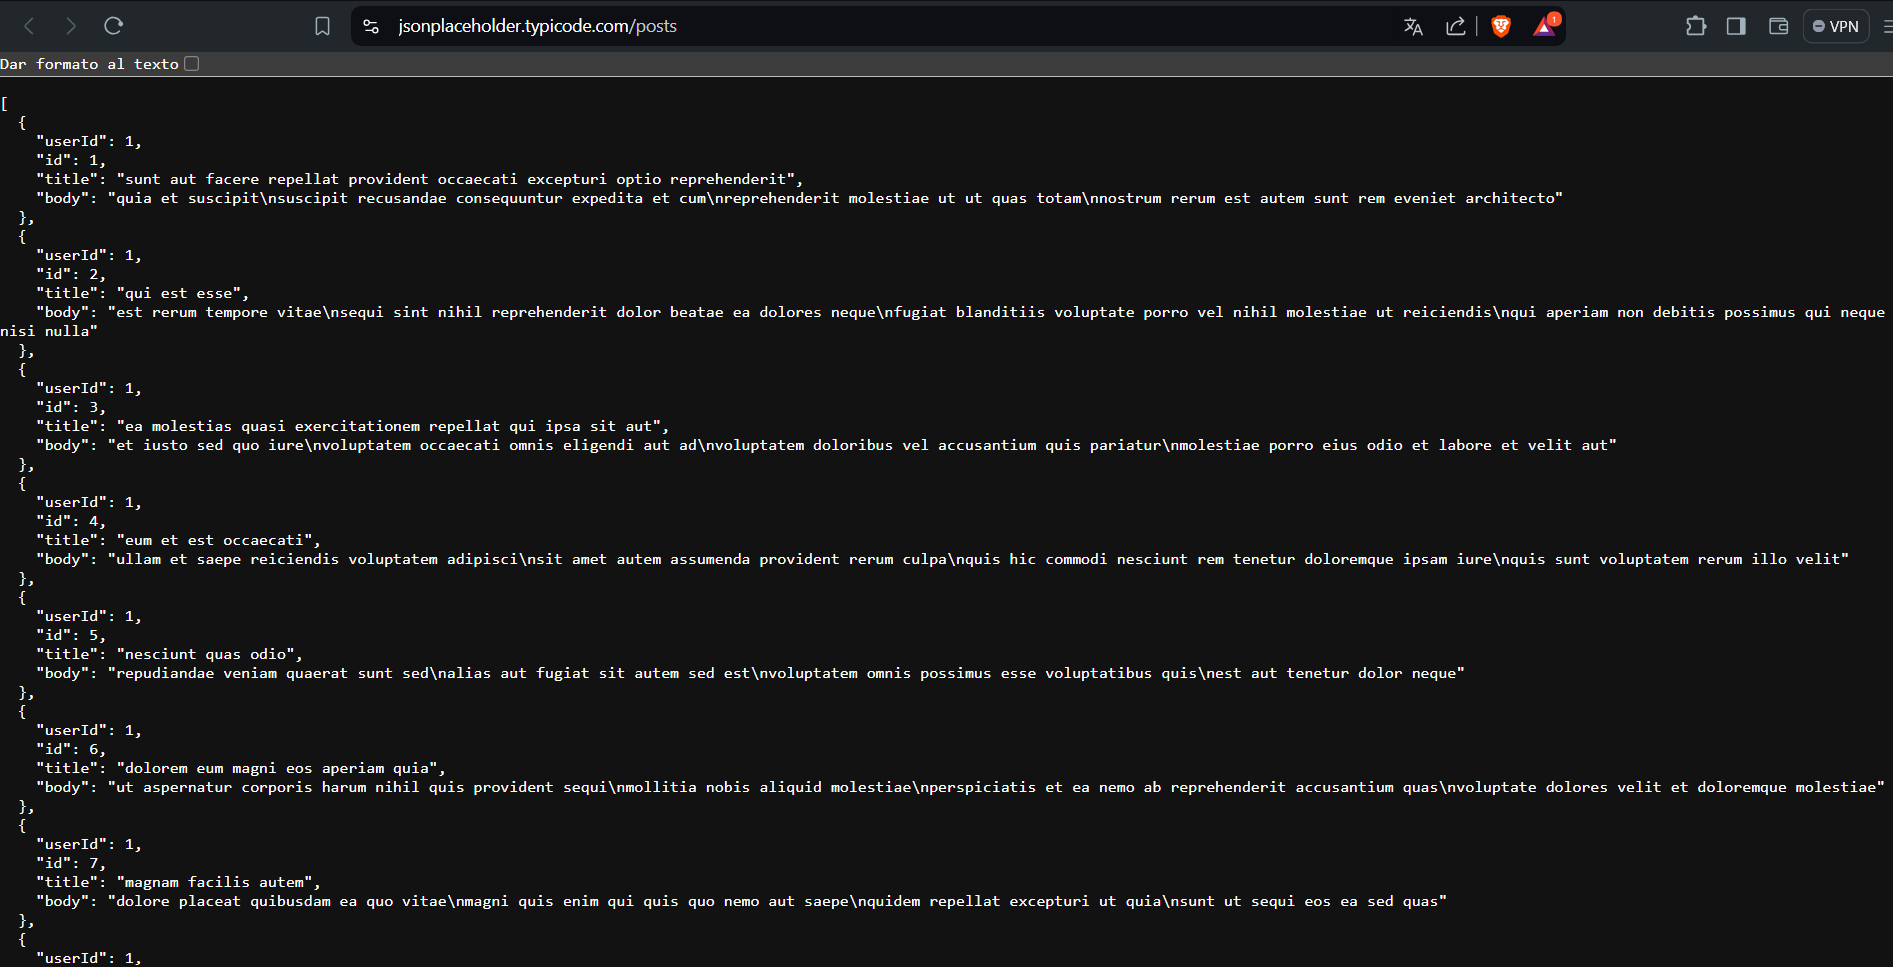
\includegraphics[width=1\textwidth, keepaspectratio]{img/json.png}}
    \caption{Json de donde se obtendra los datos}
  \end{figure}
  \begin{figure}[H]
    \centering
    \fbox{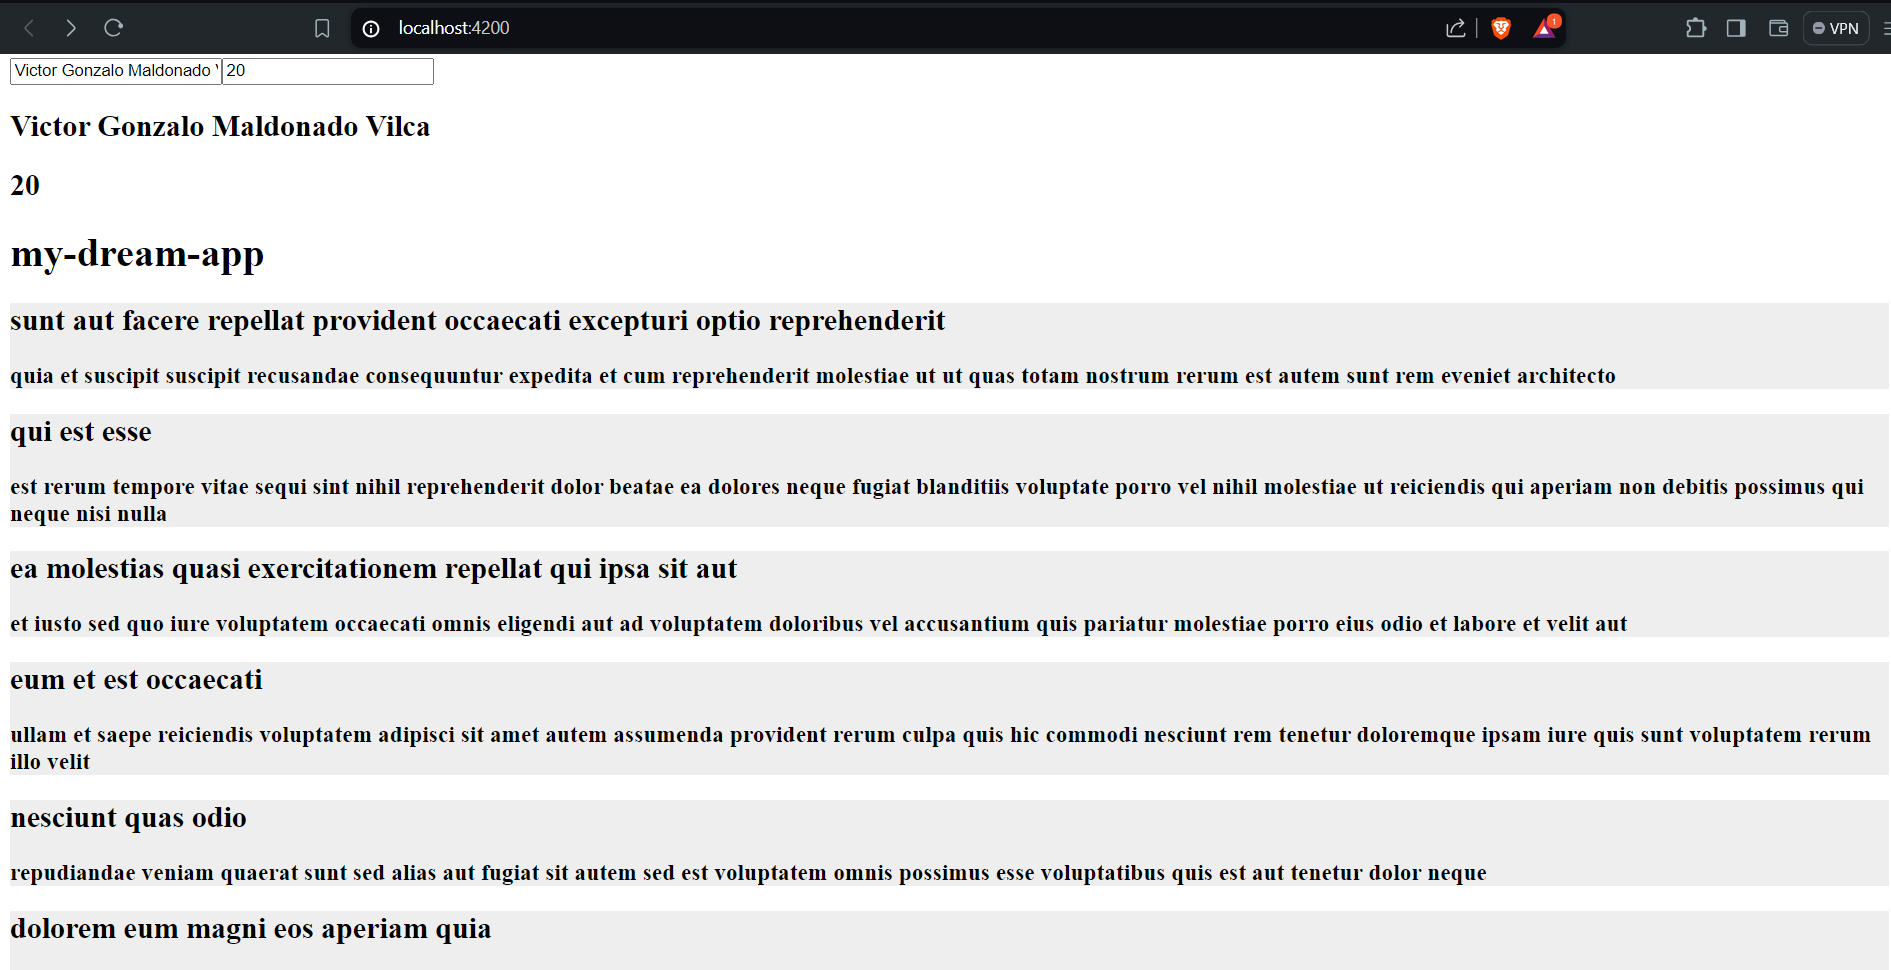
\includegraphics[width=1\textwidth, keepaspectratio]{img/ejecucion1.png}}
    \caption{Ejecución 1}
  \end{figure}
  \begin{figure}[H]
    \centering
    \fbox{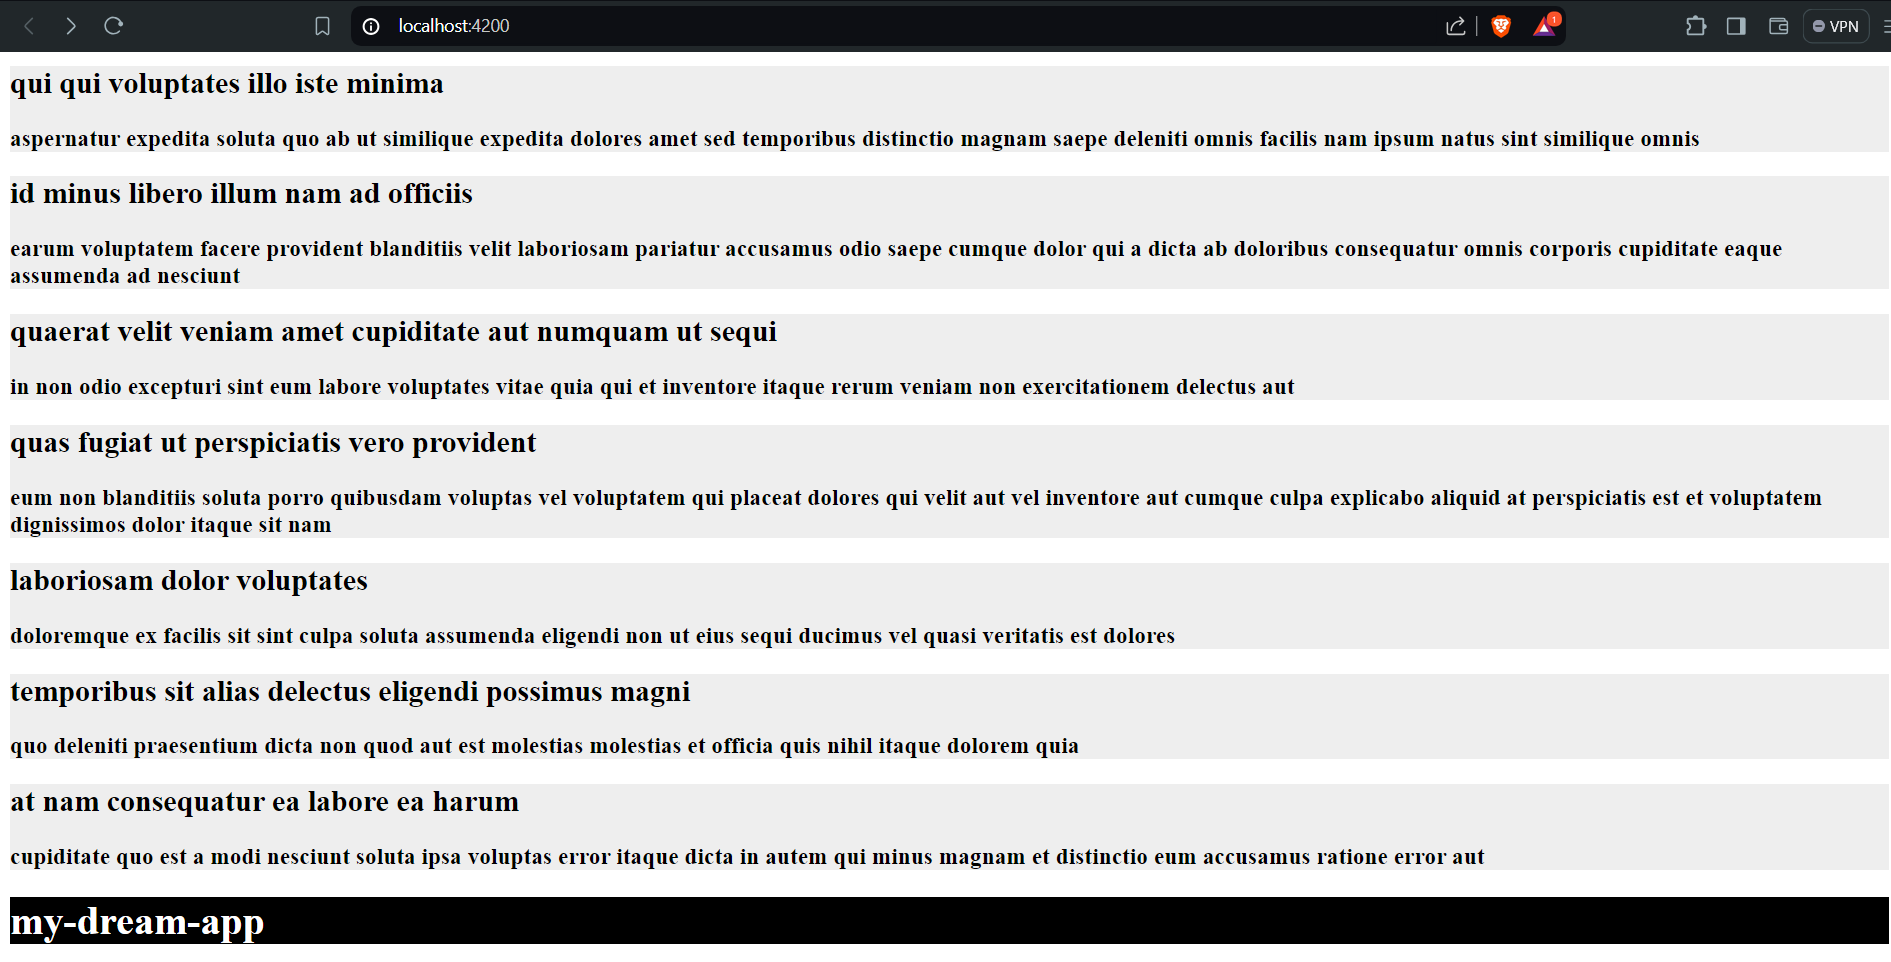
\includegraphics[width=1\textwidth, keepaspectratio]{img/ejecucion2}}
    \caption{Ejecución 2}
  \end{figure}
  \begin{figure}[H]
    \centering
    \fbox{
\includegraphics[width=1\textwidth, keepaspectratio]{img/ejecucion3}}
    \verb|\caption{Ruta "About"}|
  \end{figure}
  \begin{figure}[H]
    \centering
    \fbox{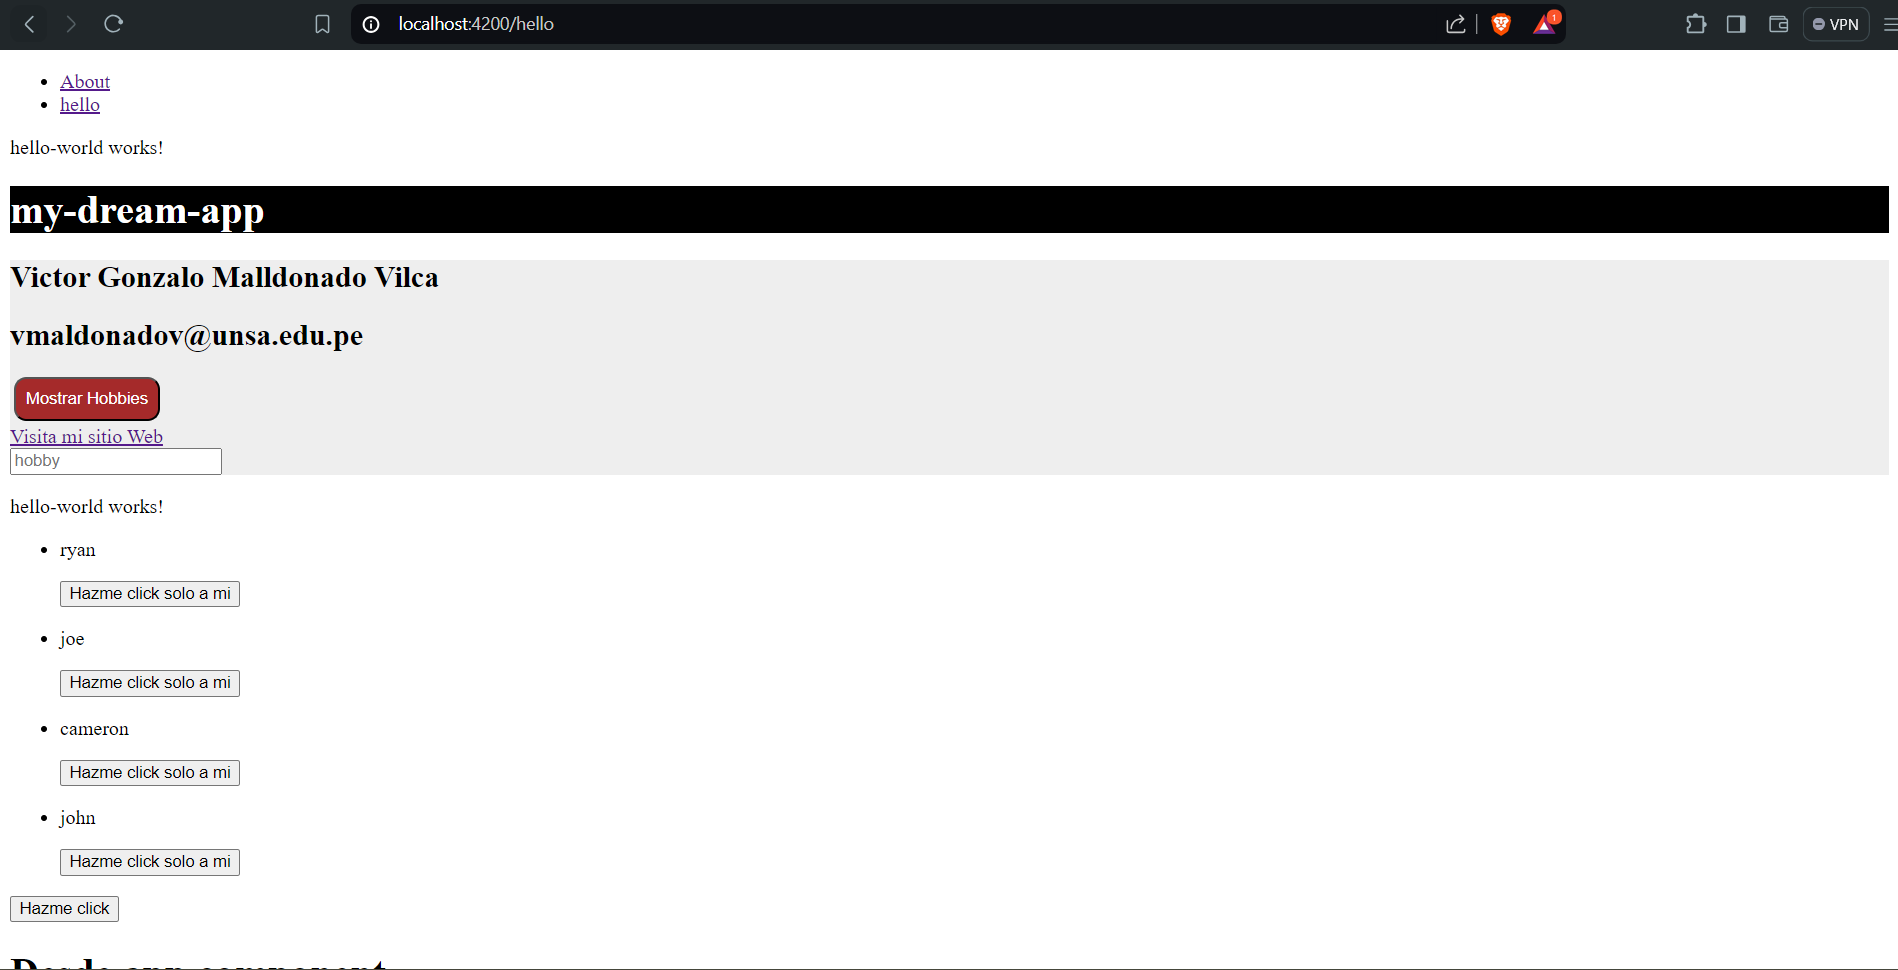
\includegraphics[width=1\textwidth, keepaspectratio]{img/ejecucion4}}
    \verb|\caption{Ruta "Hello"}|
  \end{figure}
  
%%%%%%%%%%%%

  \subsection{Componente app}
  
  \subsubsection{Archivo TypeScript}
  \begin{itemize}
    \item \textbf{Modificación del constructor: }El código ilustra cómo se emplea el servicio DataService para obtener y gestionar 
    datos en un componente. El servicio se integra en el componente mediante la inyección de dependencias 
    (private dataService: DataService). Dentro del constructor del componente, se realiza la inicialización de 
    variables como name, email, webpage, hobbies, y showHobbies. Además, se accede al método getData() del servicio, 
    el cual devuelve un Observable que se suscribe para obtener los datos 
    \newline
    \verb|(this.dataService.getData().subscribe(data => { this.posts = data; });)|. 
    Este enfoque demuestra cómo Angular maneja la recuperación de datos de forma asincrónica mediante servicios dedicados.
    \begin{lstlisting}[language=java, numbers=left, firstnumber=17, numberstyle=\color{black}]
    //Angular 2
    posts: any = [];
    
    //Angular 2
    constructor(private dataService: DataService){
      console.log('Constructor Working...');
      this.name = 'Victor Gonzalo Malldonado Vilca';
      this.email = 'vmaldonadov@unsa.edu.pe';
      this.webpage = 'http://www.unsa.edu.pe';
      this.hobbies = ['Futbol', 'Programacion', 'Netflix'];
      this.showHobbies = false;
      //Angular 2
      this.dataService.getData().subscribe(data => {
        //console.log(data);
        this.posts = data;
      });
    }
    \end{lstlisting}
    \item \textbf{Definir variables: }se define una variable name1 de tipo string que almacena el nombre.
    \newline
    \verb|{"Victor Gonzalo Maldonado Vilca"}|, y una variable age de tipo number con el valor inicial de 20. 
    \begin{lstlisting}[language=java, numbers=left, firstnumber=66, numberstyle=\color{black}]
    //Angular 2
    name1: string = "Victor Gonzalo Maldonado Vilca";
    age: number = 20;
    \end{lstlisting}
  \end{itemize}
  
  \subsubsection{Archivo html}
  \begin{itemize}
    \item \textbf{Navegación entre rutas: }Utiliza elementos de lista \verb|(<ul>)| para crear una lista desordenada 
    con dos elementos de lista \verb|(<li>)|. Cada elemento de lista contiene un enlace \verb|(<a>)| que utiliza el atributo 
    routerLink para dirigir a diferentes rutas dentro de la aplicación. Uno de los enlaces apunta a la ruta /about 
    y el otro a la ruta /hello.
    \begin{lstlisting}[language=html, numbers=left, firstnumber=1, numberstyle=\color{orange}]
    <!--Angular 2-->
    <ul>
      <li><a routerLink="/about">About</a></li>
      <li><a routerLink="/hello">hello</a></li>
    </ul>
    \end{lstlisting}
    \item \textbf{Formulario de entrada: }Esta sección contiene un formulario HTML que permite al usuario introducir 
    un nombre y una edad. Utiliza el binding bidireccional de Angular ([(ngModel)]) para enlazar los valores de los 
    campos de entrada con las propiedades name1 y age en el componente TypeScript. Los valores ingresados se muestran 
    debajo del formulario en etiquetas \verb|<h2>|.
    \begin{lstlisting}[language=html, numbers=left, firstnumber=53, numberstyle=\color{orange}]
    <!--Angular 2-->
    <div>
      <form>
        <input type='text' name='name' [(ngModel)]='name1'>
        <input type='text' name='age' [(ngModel)]='age'>
      </form>
      <h2>{{ name1 }}</h2>
      <h2>{{ age }}</h2>
    </div>
    \end{lstlisting}
    \item \textbf{Título de la Aplicación: }Esta sección simplemente muestra el valor de la propiedad title del componente 
    en una etiqueta \verb|<h1>|.
    \begin{lstlisting}[language=html, numbers=left, firstnumber=63, numberstyle=\color{orange}]
    <div>
      <h1>{{ title }}</h1>
    </div>
    \end{lstlisting}
    \item \textbf{Lista de Publicaciones: }Esta sección utiliza la directiva *ngFor de Angular para iterar 
    sobre un array de publicaciones (posts). Para cada publicación en el array, se crea un div con la clase 
    ash que contiene el título y el cuerpo de la publicación, mostrados en etiquetas \verb|<h2>| y \verb|<h3>|, respectivamente.
    \begin{lstlisting}[language=html, numbers=left, firstnumber=66, numberstyle=\color{orange}]
    <div class="ash" *ngFor="let post of posts">
      <h2>{{ post.title }}</h2>
      <h3>{{ post.body }}</h3>
    </div>
    \end{lstlisting}
  \end{itemize}
  
%%%%%%%%%%%%

  \subsection{Componente About}
  \subsubsection{Archivo html}
  \begin{itemize}
    \item \textbf{Descripción: }El fragmento HTML representa una sección \verb|"About"| con un título \verb|<h3>| y un párrafo \verb|<p>| que contiene 
    varias líneas de texto descriptivo.
    \item \textbf{Código: }
    \begin{lstlisting}[language=html, numbers=left, firstnumber=1, numberstyle=\color{orange}]
    <h3>About</h3>
    <p>enim et ex nulla\nomnis voluptas quia qui\nvoluptatem 
      consequatur numquam aliquam sunt\ntotam recusandae id 
      dignissimos aut sed asperiores deserunt</p>
    \end{lstlisting}
  \end{itemize}

  \subsubsection{Servicio data}
  \begin{itemize}
    \item \textbf{Descripción: }La clase DataService está diseñada para gestionar la obtención de datos en una 
    aplicación Angular. El constructor de esta clase toma un parámetro httpClient del tipo HttpClient, que se inyecta 
    automáticamente por Angular cuando se crea una instancia de este servicio. El constructor también incluye una 
    llamada a console.log para confirmar que el servicio está funcionando. La clase define un método getData, que 
    utiliza el httpClient para realizar una solicitud HTTP GET a la URL \url{https://jsonplaceholder.typicode.com/posts}. 
    Este método devuelve un observable que emite un array de objetos de tipo Post, permitiendo que otros componentes 
    de la aplicación se suscriban a los datos cuando estén disponibles.
    \newpage
    \item \textbf{Código: }
    \begin{lstlisting}[language=java, numbers=left, firstnumber=9, numberstyle=\color{black}]
    export class DataService {

      constructor(private httpClient:HttpClient) { 
        console.log("Service working...");
      }
      
      getData() {
        return this.httpClient.get<Post[]>("https://jsonplaceholder.typicode.com/posts");
      }
    }
    \end{lstlisting}
  \end{itemize}

  \subsubsection{Interface Post.ts}
  \begin{itemize}
    \item \textbf{Descripción: }La interfaz Post define la estructura de los objetos que representan publicaciones 
    en la aplicación. Contiene cuatro propiedades: userId, id, title y body, todas obligatorias. userId y id son 
    de tipo number, mientras que title y body son de tipo string.
    \item \textbf{Código: }
    \begin{lstlisting}[language=java, numbers=left, firstnumber=1, numberstyle=\color{black}]
    export interface Post{
      "userId" : number;
      "id" : number;
      "title" : string;
      "body" : string;
    }
    \end{lstlisting}
  \end{itemize}

  \subsubsection{Rutas}
  \begin{itemize}
    \item \textbf{Descripción: }Se define un arreglo de rutas para la aplicación. Cada ruta incluye un path 
    (ruta de la URL) y un component (componente que se carga al acceder a esa ruta). Las rutas especificadas 
    son la ruta raíz, que carga AppComponent, la ruta about, que carga AboutComponent, y la ruta hello, que 
    carga HelloWorldComponent.
    \item \textbf{Código: }
    \begin{lstlisting}[language=java, numbers=left, firstnumber=7, numberstyle=\color{black}]
    const routes: Routes = [
      {path: '', component: AppComponent},
      {path: 'about', component: AboutComponent},
      {path: 'hello', component: HelloWorldComponent},
    ];
    \end{lstlisting}
  \end{itemize}
  
%%%%%%%%%%%%

  \subsection{Visualización de otras aplicaciones de Angular}
  \begin{itemize}
    \item \textbf{Incorporación de Videos:} Angular permite la fácil integración de videos en las aplicaciones, 
    ya sea a través de componentes personalizados o utilizando servicios externos. Esto es útil para agregar 
    contenido multimedia enriquecido que mejore la experiencia del usuario.
    \item \textbf{Integración con Bootstrap:} Utilizando Bootstrap con Angular, los desarrolladores pueden crear 
    interfaces de usuario receptivas y atractivas de manera eficiente. Bootstrap proporciona un conjunto de componentes 
    predefinidos y estilos que se pueden personalizar e integrar sin problemas en las aplicaciones Angular.
    \item \textbf{Interoperabilidad con Django:} Angular puede funcionar junto con Django para crear aplicaciones 
    web robustas y escalables. Mientras que Django maneja el backend y la lógica del servidor, Angular se encarga 
    del frontend, proporcionando una experiencia de usuario fluida y dinámica.
  \end{itemize}


%%%%%%%%%%%%%%%%%%%%

  \section{Conclusiones}
  \begin{itemize}
    \item La configuración de rutas en Angular es fundamental para la navegación dentro de una aplicación.
    \item Definir rutas claras y asignarles componentes específicos permite una mejor organización y accesibilidad 
    de las diferentes partes de la aplicación.
    \item Utilizar componentes separados para distintas rutas ayuda a mantener el código modular y más fácil de mantener.
    \item Este enfoque también facilita la implementación de nuevas funcionalidades y mejora la experiencia del 
    usuario al navegar por la aplicación.
    \item Seguir una estructura bien definida para las rutas asegura que la aplicación sea escalable y manejable 
    a medida que crece en complejidad.
    \item El uso de servicios como \texttt{DataService} permite la obtención de datos de fuentes externas, como una 
    API, y la integración de estos datos en la aplicación.
    \item Emplear interfaces como \texttt{Post} para definir la estructura de los datos recibidos garantiza que los datos 
    se manejen de manera consistente y tipada, lo que mejora la seguridad y la legibilidad del código.
    \item La interacción con APIs RESTful, como la obtención de datos desde \url{https://jsonplaceholder.typicode.com/posts}, 
    demuestra la capacidad de Angular para manejar datos dinámicos y actualizaciones en tiempo real.
    \item Integrar datos JSON en la aplicación permite a los desarrolladores trabajar con datos estructurados de manera 
    eficiente, facilitando tareas como la visualización de listas y la gestión de información en la interfaz de usuario.
  \end{itemize}



%%%%%%%%%%%%%%%%%%%%
	\newpage
	\subsection{\textcolor{red}{Rúbrica para el contenido del Informe y demostración}}
	\begin{itemize}			
		\item El alumno debe marcar o dejar en blanco en celdas de la columna \textbf{Checklist} si cumplio con el ítem correspondiente.
		\item Si un alumno supera la fecha de entrega,  su calificación será sobre la nota mínima aprobada, siempre y cuando cumpla con todos lo items.
		\item El alumno debe autocalificarse en la columna \textbf{Estudiante} de acuerdo a la siguiente tabla:
	
		\begin{table}[ht]
			\caption{Niveles de desempeño}
			\begin{center}
			\begin{tabular}{ccccc}
    			\hline
    			 & \multicolumn{4}{c}{Nivel}\\
    			\cline{1-5}
    			\textbf{Puntos} & Insatisfactorio 25\%& En Proceso 50\% & Satisfactorio 75\% & Sobresaliente 100\%\\
    			\textbf{2.0}&0.5&1.0&1.5&2.0\\
    			\textbf{4.0}&1.0&2.0&3.0&4.0\\
    		\hline
			\end{tabular}
		\end{center}
	\end{table}	
	

	\end{itemize}

 
	
	\begin{table}[H]
		\caption{Rúbrica para contenido del Informe y demostración}
		\setlength{\tabcolsep}{0.5em} % for the horizontal padding
		{\renewcommand{\arraystretch}{1.5}% for the vertical padding
		%\begin{center}
		\begin{tabular}{|p{2.7cm}|p{7cm}|x{1.3cm}|p{1.2cm}|p{1.5cm}|p{1.1cm}|}
			\hline
    		\multicolumn{2}{|c|}{Contenido y demostración} & Puntos & Checklist & Estudiante & Profesor\\
			\hline
			\textbf{1. GitHub} & Hay enlace URL activo del directorio para el  laboratorio hacia su repositorio GitHub con código fuente terminado y fácil de revisar. &2 &X &2 & \\ 
			\hline
			\textbf{2. Commits} &  Hay capturas de pantalla de los commits más importantes con sus explicaciones detalladas. (El profesor puede preguntar para refrendar calificación). &4 &X &4 & \\ 
			\hline 
			\textbf{3. Código fuente} &  Hay porciones de código fuente importantes con numeración y explicaciones detalladas de sus funciones. &2 &X &2 & \\ 
			\hline 
			\textbf{4. Ejecución} & Se incluyen ejecuciones/pruebas del código fuente  explicadas gradualmente. &2 &X &2 & \\ 
			\hline			
			\textbf{5. Pregunta} & Se responde con completitud a la pregunta formulada en la tarea.  (El profesor puede preguntar para refrendar calificación).  &2 &X &2 & \\ 
			\hline	
			\textbf{6. Fechas} & Las fechas de modificación del código fuente estan dentro de los plazos de fecha de entrega establecidos. &2 &X &2 & \\ 
			\hline 
			\textbf{7. Ortografía} & El documento no muestra errores ortográficos. &2 &X &2 & \\ 
			\hline 
			\textbf{8. Madurez} & El Informe muestra de manera general una evolución de la madurez del código fuente,  explicaciones puntuales pero precisas y un acabado impecable.   (El profesor puede preguntar para refrendar calificación).  &4 &X &4 & \\ 
			\hline
			\multicolumn{2}{|c|}{\textbf{Total}} &20 & &20 & \\ 
			\hline
		\end{tabular}
		%\end{center}
		%\label{tab:multicol}
		}
	\end{table}


%%%%%%%%%%%%%%%%%%%%%%%%%%%%%%%%%%%%%%%%%%%%%%%%%%%%%%%%%%%%%%%%%%%
	
  \newpage
  \section{Referencias}
  \begin{itemize}
    \item \url{https://v17.angular.io/guide/architecture}
    \item \url{https://v17.angular.io/guide/binding-syntax}
  \end{itemize}

%%%%%%%%%%%%%%%%%%%% 
%\clearpage
%\bibliographystyle{apalike}
%\bibliographystyle{IEEEtranN}
%\bibliography{bibliography}
			
\end{document}
